\documentclass[a4paper]{article}
\usepackage[utf8]{inputenc}
\usepackage{amsthm, amsmath, mathtools, amssymb}
\usepackage[left=2cm,right=2cm,top=2cm,bottom=2cm]{geometry}
\usepackage[colorlinks,linkcolor=blue,citecolor=blue,urlcolor=blue]{hyperref}
\usepackage{array}
\usepackage[catalan,english]{babel}
\usepackage[affil-it]{authblk}
\usepackage{titlesec}
\usepackage[intlimits]{esint} % for more options on integrals.
\usepackage{physics}
\usepackage[hypcap=false]{caption}
\usepackage{subcaption}
\usepackage{multirow}
% \titleformat{\section}
%   {\normalfont\fontsize{13}{15}\bfseries}{\thesection}{1em}{}

\newcommand{\NN}{\ensuremath{\mathbb{N}}} % set of natural numbers
\newcommand{\ZZ}{\ensuremath{\mathbb{Z}}} % set of integers
\newcommand{\QQ}{\ensuremath{\mathbb{Q}}} % set of rationals
\newcommand{\RR}{\ensuremath{\mathbb{R}}} % set of real numbers
\newcommand{\CC}{\ensuremath{\mathbb{C}}} % set of complex numbers
\newcommand{\KK}{\ensuremath{\mathbb{K}}} % a general field

\newcommand{\vf}[1]{\boldsymbol{\mathrm{#1}}} % math style for vectors and matrices and vector-values functions (previously it was \*vb{#1} but this does not apply to greek letters)
\newcommand{\ii}{\mathrm{i}} % imaginary unit
\newtheorem{theorem}{Teorema}
\newtheorem{prop}{Proposició}
\theoremstyle{definition}
\newtheorem{definition}{Definició}
\DeclareDocumentCommand\derivative{ s o m g d() }{ 
  % Total derivative
  % s: star for \flatfrac flat derivative
  % o: optional n for nth derivative
  % m: mandatory (x in df/dx)
  % g: optional (f in df/dx)
  % d: long-form d/dx(...)
    \IfBooleanTF{#1}
    {\let\fractype\flatfrac}
    {\let\fractype\frac}
    \IfNoValueTF{#4}
    {
        \IfNoValueTF{#5}
        {\fractype{\diffd \IfNoValueTF{#2}{}{^{#2}}}{\diffd #3\IfNoValueTF{#2}{}{^{#2}}}}
        {\fractype{\diffd \IfNoValueTF{#2}{}{^{#2}}}{\diffd #3\IfNoValueTF{#2}{}{^{#2}}} \argopen(#5\argclose)}
    }
    {\fractype{\diffd \IfNoValueTF{#2}{}{^{#2}} #3}{\diffd #4\IfNoValueTF{#2}{}{^{#2}}}\IfValueT{#5}{(#5)}}
} % differential operator
\DeclareDocumentCommand\partialderivative{ s o m g d() }{ 
  % Total derivative
  % s: star for \flatfrac flat derivative
  % o: optional n for nth derivative
  % m: mandatory (x in df/dx)
  % g: optional (f in df/dx)
  % d: long-form d/dx(...)
  \IfBooleanTF{#1}
    {\let\fractype\flatfrac}
    {\let\fractype\frac}
    \IfNoValueTF{#4}{
      \IfNoValueTF{#5}
      {\fractype{\partial \IfNoValueTF{#2}{}{^{#2}}}{\partial #3\IfNoValueTF{#2}{}{^{#2}}}}
      {\fractype{\partial \IfNoValueTF{#2}{}{^{#2}}}{\partial #3\IfNoValueTF{#2}{}{^{#2}}} \argopen(#5\argclose)}
    }
    {\fractype{\partial \IfNoValueTF{#2}{}{^{#2}} #3}{\partial #4\IfNoValueTF{#2}{}{^{#2}}}\IfValueT{#5}{(#5)}}
} % partial differential operator

\renewcommand{\labelenumii}{\alph{enumii})}

\title{\bfseries\large SEMINARI 1}

\author{Víctor Ballester Ribó\endgraf NIU:1570866}
\date{\parbox{\linewidth}{\centering
  Sistemes dinàmics\endgraf
  Grau en Matemàtiques\endgraf
  Universitat Autònoma de Barcelona\endgraf
  Desembre de 2022}}

\setlength{\parindent}{0pt}
\begin{document}
\selectlanguage{catalan}
\maketitle
\section{\texorpdfstring{Osci\lgem ador}{Oscil.lador} de Van der Pol}
Considerem el sistema diferencial:
\begin{equation}\label{sis1}
  x''-\mu(1-x^2)x'+x=0\iff\left\{
  \begin{aligned}
    x' & =y                & =:  f_1(x,y) \\
    y' & =-x + \mu(1-x^2)y & =: f_2(x,y)
  \end{aligned}
  \right.
\end{equation}
amb $\mu\in\RR$. Fixem-nos que el sistema és invariant pel canvi $(x,y,\mu, t)\to(z,-y,-\mu,-t)$. Per tant, podem restringir el nostre estudi a $\mu>0$. Observem d'altra banda que el nostre sistema es tracta d'un sistema de Liénard. El teorema de Liénard ens assegura l'existència d'un únic cicle límit per $\forall\mu>0$:
\begin{theorem}
  Sigui $F,g\in \mathcal{C}^1(\RR)$ funcions senars tal que:
  \begin{itemize}
    \item $xg(x)>0$ per $x\ne 0$.
    \item $F'(0)<0$.
    \item $F$ té un únic zero positiu a $x=a$.
    \item $F$ creix monòtonament cap a infinit per $x\geq a$ quan $x\to\infty$.
  \end{itemize}
  Llavors, el sistema de Liénard
  \begin{equation}
    x''+f(x)x'+g(x)=0\iff\left\{
    \begin{aligned}
      x' & =y-F(x) \\
      y' & =-g(x)
    \end{aligned}
    \right.
  \end{equation}
  té exactament un cicle límit i és estable.
\end{theorem}
En efecte, en el nostre cas $F$ és una primitiva de la funció $f(x) =-\mu (1-x^2)$, que ha de ser senar. Per tant, hem de prendre $F(x)=-\mu(x-\frac{x^3}{3})$. D'alta banda, $g(x) = x$ també és senar i satisfà $xg(x)>0$ $\forall x\ne 0$. A més, $F'(0)=f(0)=-\mu <0$, $F$ té un únic zero positiu en $x=\sqrt{3}>1$ i $F'(x)=f(x)>0$ per $x\geq \sqrt{3}$. Per tant, pel teorema de Liénard, sabem que existeix un únic cicle límit pel nostre sistema.

Ara recordem el teorema de Melinikov de perturbacions de sistemes Hamiltonians:
\begin{theorem}
  Siguin $H,P,Q\in\mathcal{C}^1(\RR)$ i $\varepsilon\simeq 0$. Considerem el següent sistema diferencial:
  \begin{equation*}
    \left\{
    \begin{aligned}
      x' & =-H_y +\varepsilon P(x,y) \\
      y' & =H_x +\varepsilon Q(x,y)
    \end{aligned}
    \right.
  \end{equation*}
  Sigui $\vf\gamma_h=\{H(x,y)=h\in\RR\}$ i definim la següent funció: $$M(h)=\int_{\vf\gamma_h}Q\dd{x}-P\dd{y}$$ Si $M$ té un zero simple en $h=h^*$, aleshores existeix un cicle límit $\vf\Gamma_\varepsilon$ per $\varepsilon\simeq 0$ tal que $\displaystyle\lim_{\varepsilon\to 0}\vf\Gamma_\varepsilon=\vf\gamma_{h^*}$.
\end{theorem}
El nostre sistema és una pertorbació d'un sistema Hamiltonià amb $H(x,y) = x^2+y^2$, $P(x,y)=0$ i $Q(x,y) = (1-x^2)y$. Calculant la integral $M(h)$ en el nostre cas, obtenim:
$$
  M(h) = \int_{\vf\gamma_h}Q\dd{x}-P\dd{y} = -\int_{\{x^2+y^2\leq h\}}\left(\pdv{P}{x}+\pdv{Q}{y}\right)\dd{x}\dd{y}=-\int_{\{x^2+y^2\leq h\}}(1-x^2)\dd{x}\dd{y} = \frac{h\pi(h-4)}{4}
$$
on en la segona igualtat hem fet servir la fórmula de Green. Aquesta funció té un zero simple per $h=4$, que correspon al cercle de radi 2. Per tant, podem prendre com a aproximació inicial per els cicles límit $\rho\approx 2$ per a $\mu \simeq 0$ i, com que per $\mu=0$ el nostre sistema és un centre amb totes les òrbites del mateix període $2\pi$, podem prendre $T\approx 2\pi$ com a aproximació del període, per la continuïtat de les solucions respecte paràmetres.

Gràficament també podem detectar l'existència d'aquest cicle límit integrant l'equació a partir d'una condició inicial $(\rho_0, 0)$ i $(\rho_1,0)$ amb $\rho_0<2$ i $\rho_1>2$. Fent-ho, obtenim el següent resultat:

\begin{figure}[ht]
  \centering
  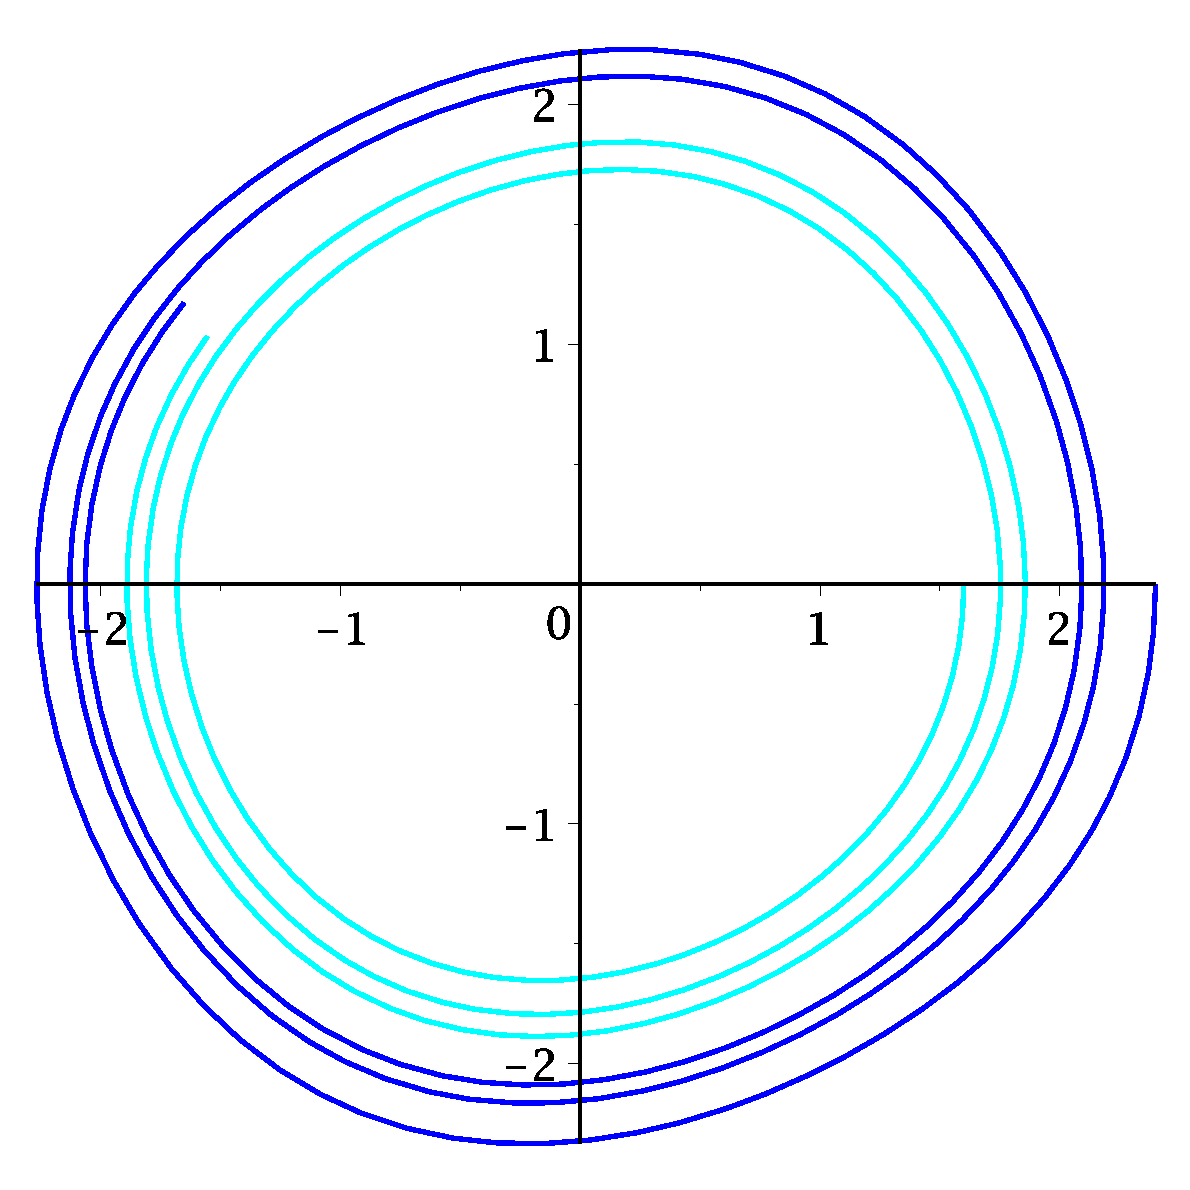
\includegraphics[width=0.5\linewidth]{Images/ex1-2sol.eps}
\end{figure}

Ens preguntem per a cada $\mu>0$ quin és el $\rho_\mu$ tal que l'òrbita periòdica passa pel punt $(\rho_\mu,0)$. Per això farem ús de l'aplicació de Poincaré $\Pi$ prenent com a secció transversal $\{y=0\}$. Així doncs, donada $\mu>0$ hem de trobar el punt fix de l'equació $\Pi_\mu(x)=x$ o, equivalentment, el zero de l'aplicació de retorn $d_\mu(x)=\Pi_\mu(x) -x$. Aquí hem denotat $\Pi_\mu$ i $d_\mu$ l'aplicació de Poincaré i de retorn, respectivament, per a cada paràmetre de $\mu$. Com que resoldrem l'equació numèricament, la nostra funció $\Pi_\mu$ no la tindrem explícita, sinó que només tindrem punts. Per tant, per tal de trobar aquest zero de $d_\mu$ ens haurem d'utilitzar el mètode de Newton-Raphson. És per això que ens cal calcular ${\Pi_\mu}'(x)$. A més. recordem que $\Pi_\mu(x)=\phi_1(T_\mu(x), (x, 0))$, on $\Phi=(\phi_1,\phi_2)$ és el flux de l'equació diferencial i $T_\mu(x)$ satisfà $\phi_2(T_\mu(x),(x,0))= 0$. Derivant implicitament aquestes dues equacions respecte $x$ deduïm que:
\begin{align}
  \nonumber 0                 & =\pdv{\phi_2}{t}{T_\mu}'(x) + \pdv{\phi_2}{x}= f_2 {T_\mu}'(x) + \pdv{\phi_2}{x} \implies {T_\mu}'(x) = -\frac{\pdv{\phi_2}{x}}{f_2} \\
  \label{eqPoin}{\Pi_\mu}'(x) & =\pdv{\phi_1}{t}{T_\mu}'(x) + \pdv{\phi_1}{x}= \pdv{\phi_1}{x} + f_1{T_\mu}'(x) =\pdv{\phi_1}{x} - \frac{f_1}{f_2} \pdv{\phi_2}{x}
\end{align}
on hem omès escriure l'avaluació a $(T_\mu(x),(x,0))$ per tal de simplificar la notació. Per tant:
$${d_\mu}'=\pdv{\phi_1}{x} - \frac{f_1}{f_2} \pdv{\phi_2}{x} - 1$$
Recordem que $\displaystyle\pdv{\vf\Phi}{x}(t,(x,y))={\left(\pdv{\phi_1}{x},\pdv{\phi_2}{x}\right)}^\mathrm{T}$ satisfà el sistema lineal d'equacions diferencials següent:
\begin{equation}
  \left\{
  \begin{aligned}
    \vf{y}'   & =\vf{Df}(t,\vf\Phi(t,(x,y)))\vf{y} \\
    \vf{y}(0) & ={(1,0)}^\mathrm{T}
  \end{aligned}
  \right.
\end{equation}
on $\vf{Df}$ és la diferencial del nostre sistema inicial. Integrant aquesta equació simultàniament amb l'equació \eqref{sis1} i fent els càlculs pertinents obtenim els següents resultats.

\hspace{2cm}

\begin{tabular}{ccc}
  \begin{minipage}[b]{0.36\linewidth}
    \centering
    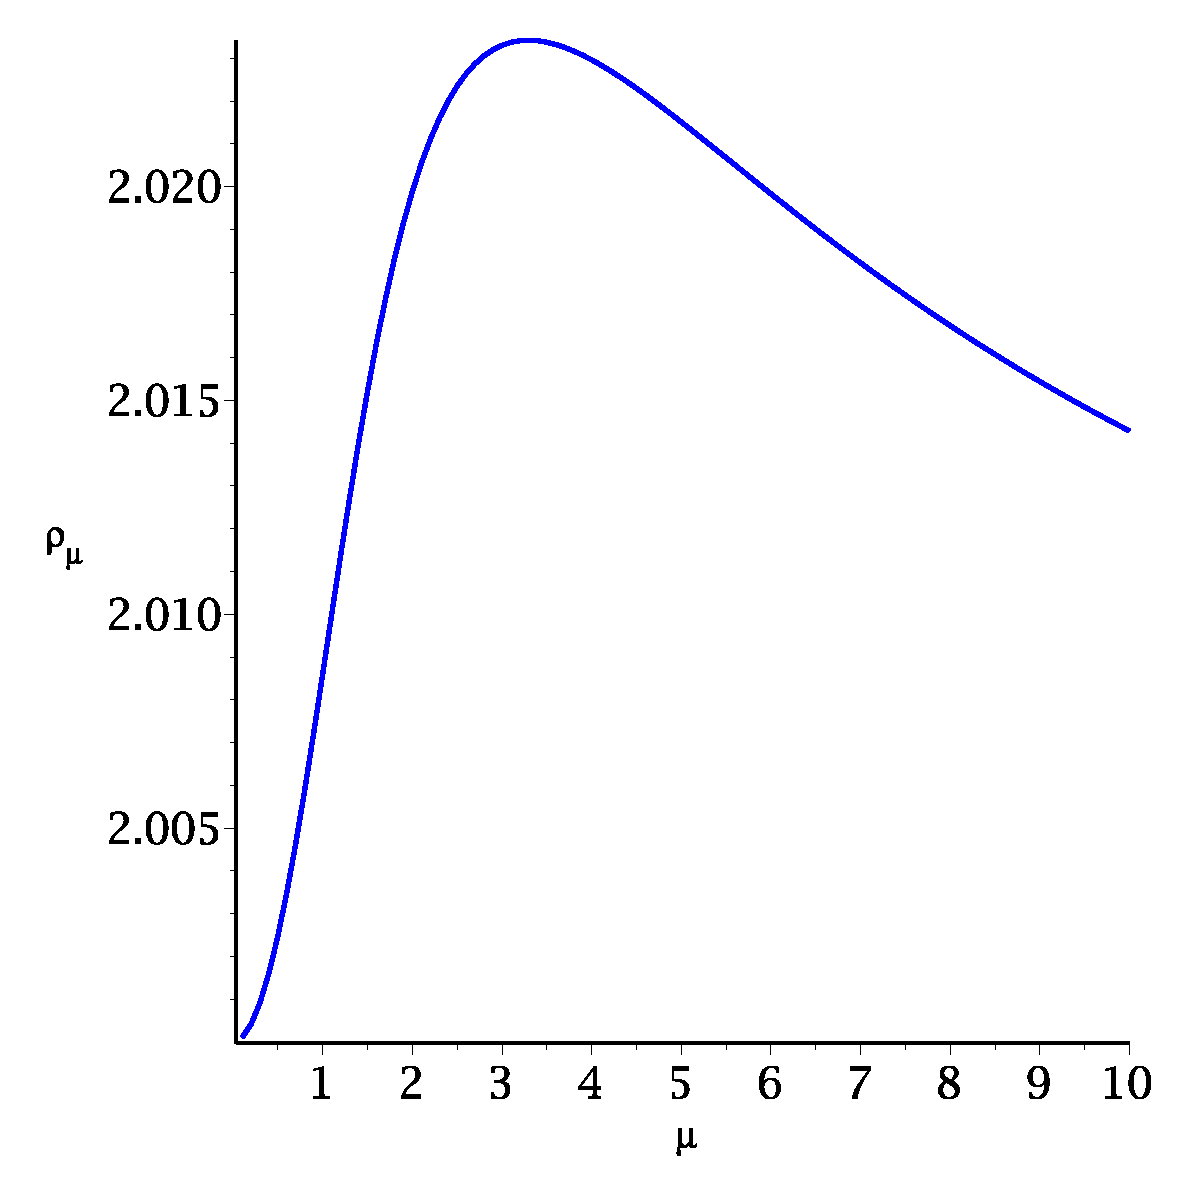
\includegraphics[width=\linewidth]{Images/mu_rho_petits.eps}
    \captionof{figure}{Gràfic de $\rho_\mu$ en funció de $\mu$ per a $\mu$'s petits}
  \end{minipage} &
  \begin{minipage}[b]{0.36\linewidth}
    \centering
    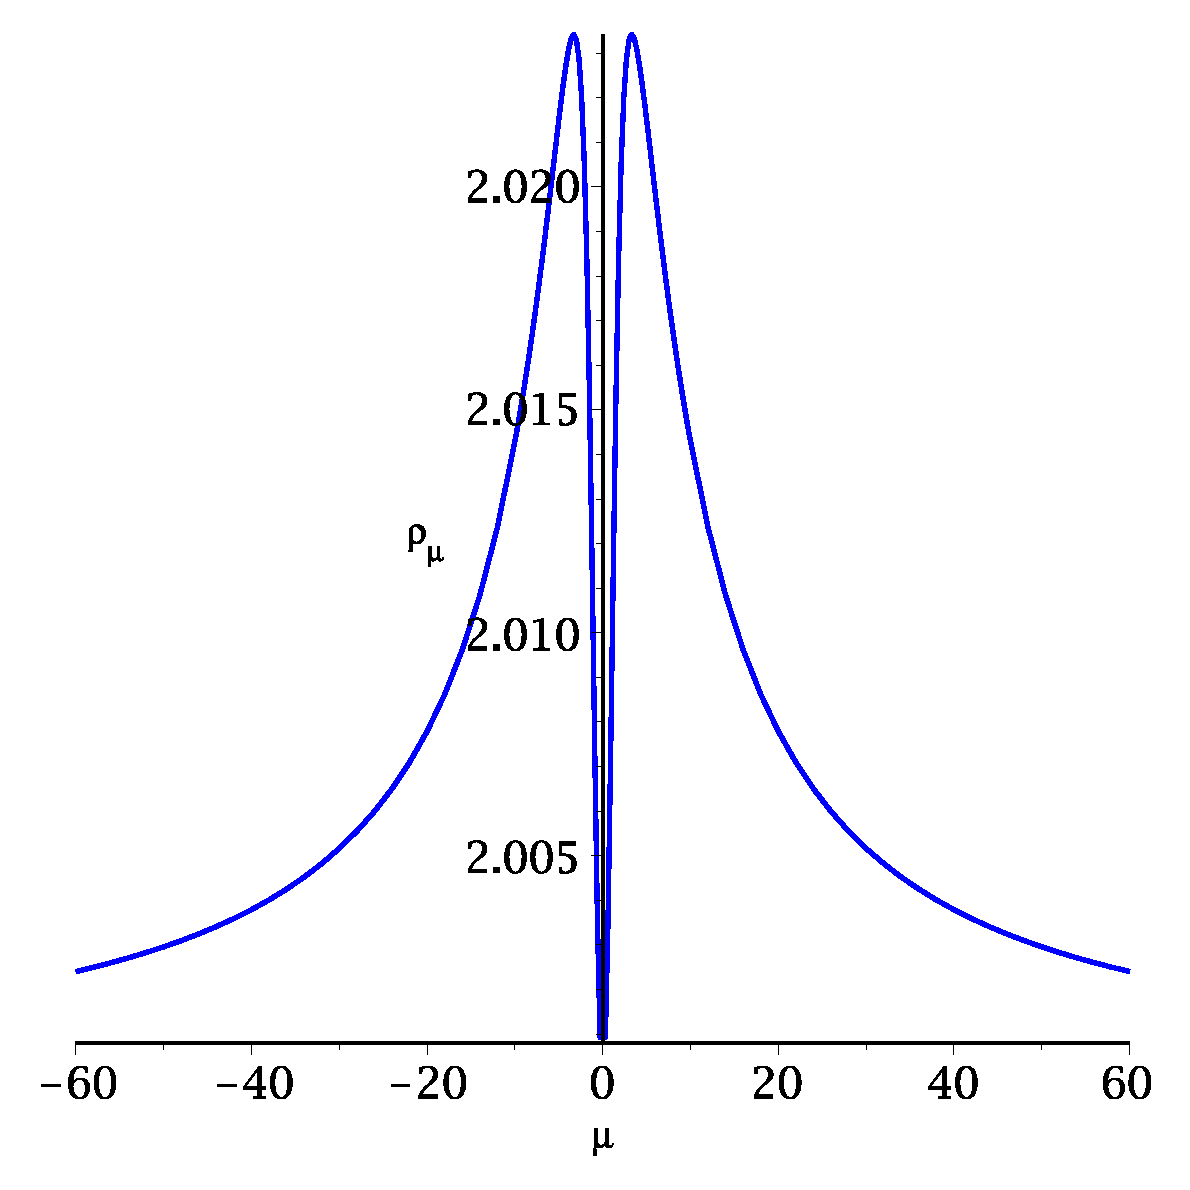
\includegraphics[width=\linewidth]{Images/mu_rho.eps}
    \captionof{figure}{Gràfic de $\rho_\mu$ en funció de $\mu$ per a $\mu$'s grans}
  \end{minipage}  & \multirow[t]{2}{*}{
    \begin{minipage}[ht]{0.18\linewidth}
      \centering
      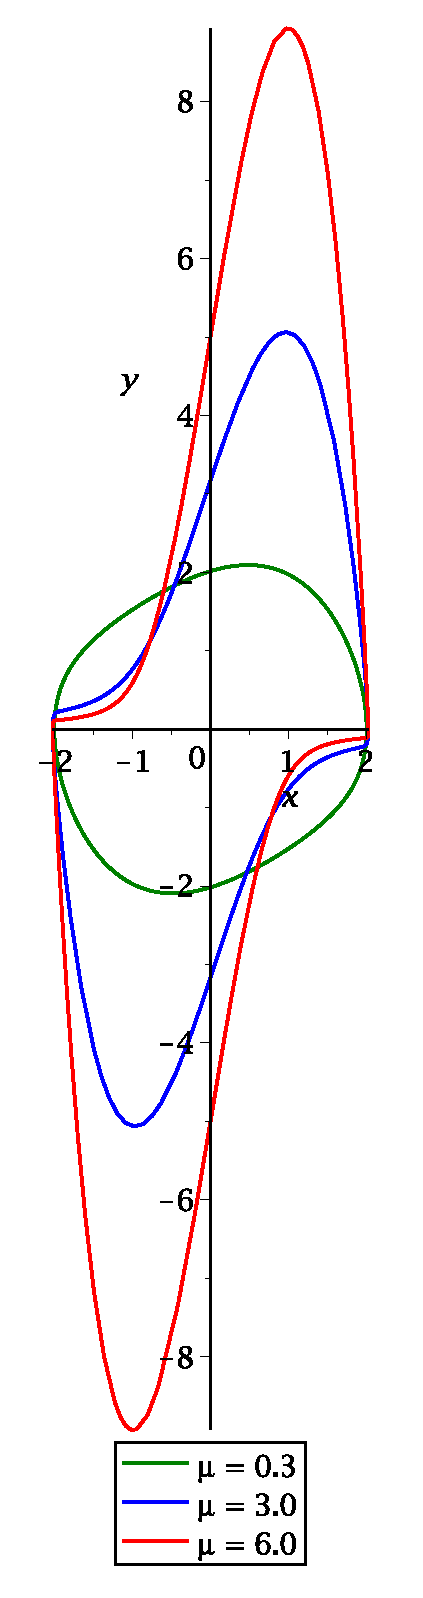
\includegraphics[width=\linewidth]{Images/ex1-op.eps}
      \captionof{figure}{Els tres cicles límit del sistema per $\mu =0.3,3,6$}
      \label{ex1_op}
    \end{minipage}
  }                                                                                  \\
  \begin{minipage}[b]{0.36\linewidth}
    \centering
    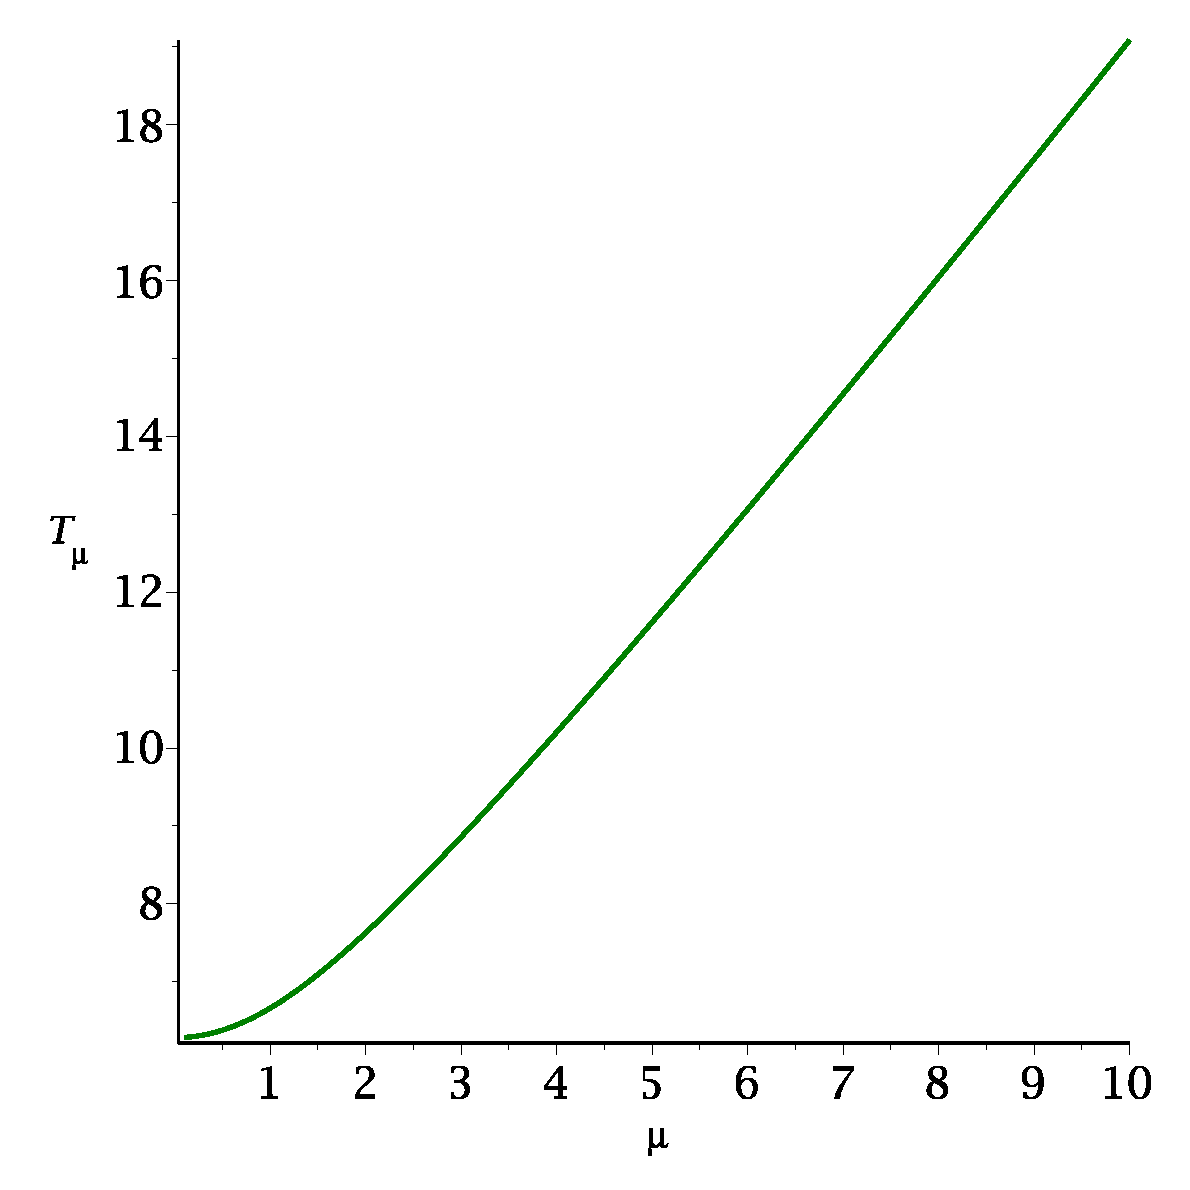
\includegraphics[width=\linewidth]{Images/mu_T_petits.eps}
    \captionof{figure}{Gràfic de $T_\mu$ en funció de $\mu$ per a $\mu$'s petits}
  \end{minipage}
                                                                                   &
  \begin{minipage}[b]{0.36\linewidth}
    \centering
    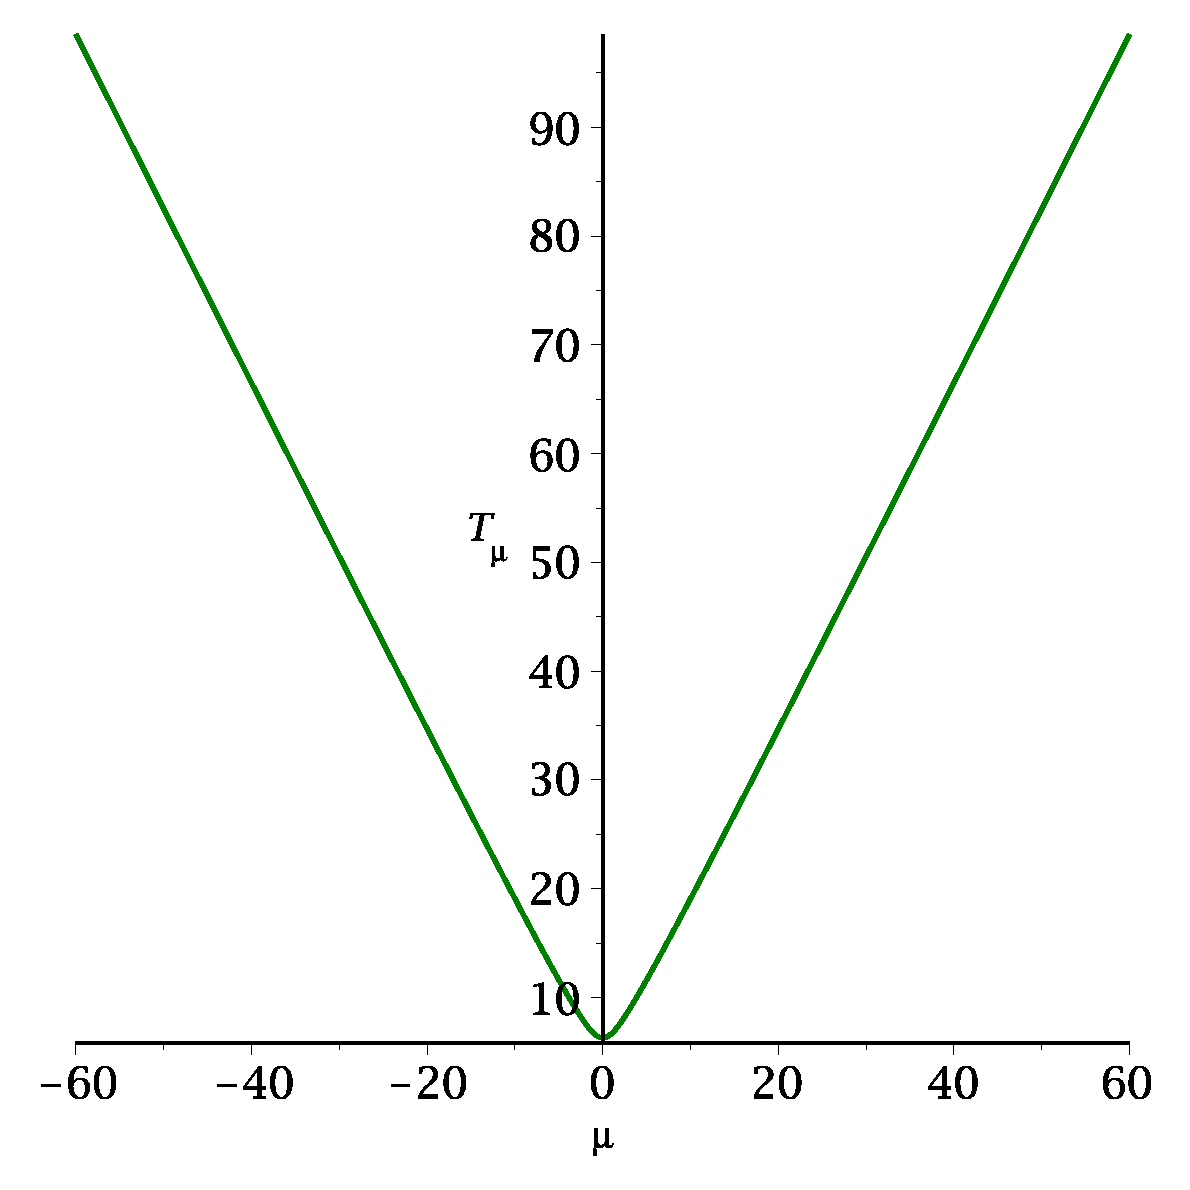
\includegraphics[width=\linewidth]{Images/mu_T.eps}
    \captionof{figure}{Gràfic de $T_\mu$ en funció de $\mu$ per a $\mu$'s grans}
  \end{minipage}     &
\end{tabular}

\hspace{2cm}

Algunes de les òrbites periòdiques que obtenim al variar $\mu$ són les que observem a la figura \ref{ex1_op}. Observem que encara que $\rho_\mu$ és aproximadament $2$ per a tota $\mu$, el període augmenta a la llarga de forma lineal degut a, en part, l'allargament de les òrbites periòdiques conforme creix $\abs{\mu}$.
\newpage
\section{Cicles límit en camps quadràtics}
Considerem el sistema diferencial:
\begin{equation}\label{sist2}
  \left\{
  \begin{aligned}
    x' & = -x +by +y^2                 \\
    y' & =ax -aby -xy +c( -x +by +y^2)
  \end{aligned}
  \right.
\end{equation}
amb $a,b,c\in\RR$. Se'ns diu que aquest sistema té una òrbita periòdica que envolta el punt crític $(x_e, y_e)=(2,2)$ quan $a=1$, $b=-1$ i $c=3/4$. Com que no tenim una estimació inicial del període de l'òrbita, ens situem sobre la recta vertical $x = 2$ i fem corre el temps fins a donar gairebé una volta per saber de quin ordre de magnitud és el temps. Fent això (veure figura \ref{eq2-intent}) obtenim que el període és $T\approx 4$ i per tant, de nou fent servir l'aplicació de Poincaré i el mètode de Newton-Raphson (descrits en el problema anterior però ara canviant la secció transversal horitzontal per una vertical) obtenim l'òrbita periòdica que s'exposa a la figura \ref{ex2-op}.

\begin{center}
  \begin{minipage}{0.4\linewidth}
    \centering
    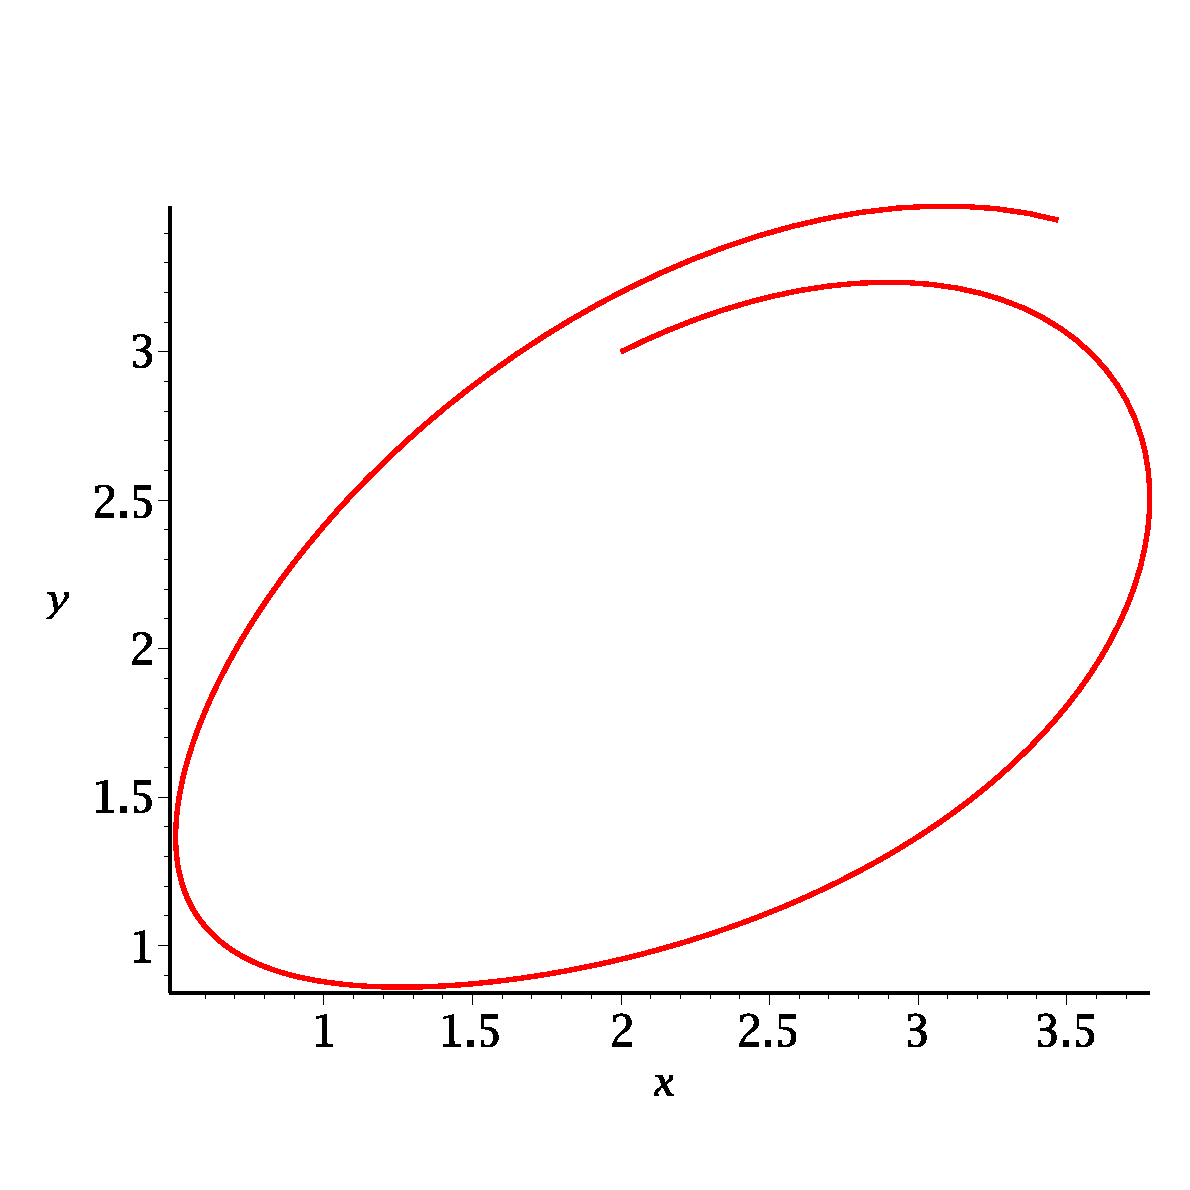
\includegraphics[width=\linewidth]{Images/ex2-intent.eps}
    \captionof{figure}{Integració del sistema partint de la condició inicial $(x,y)= (2,3)$ i deixant corre el temps des de 0 fins a 4}
    \label{eq2-intent}
  \end{minipage}
  \qquad
  \begin{minipage}{0.4\linewidth}
    \centering
    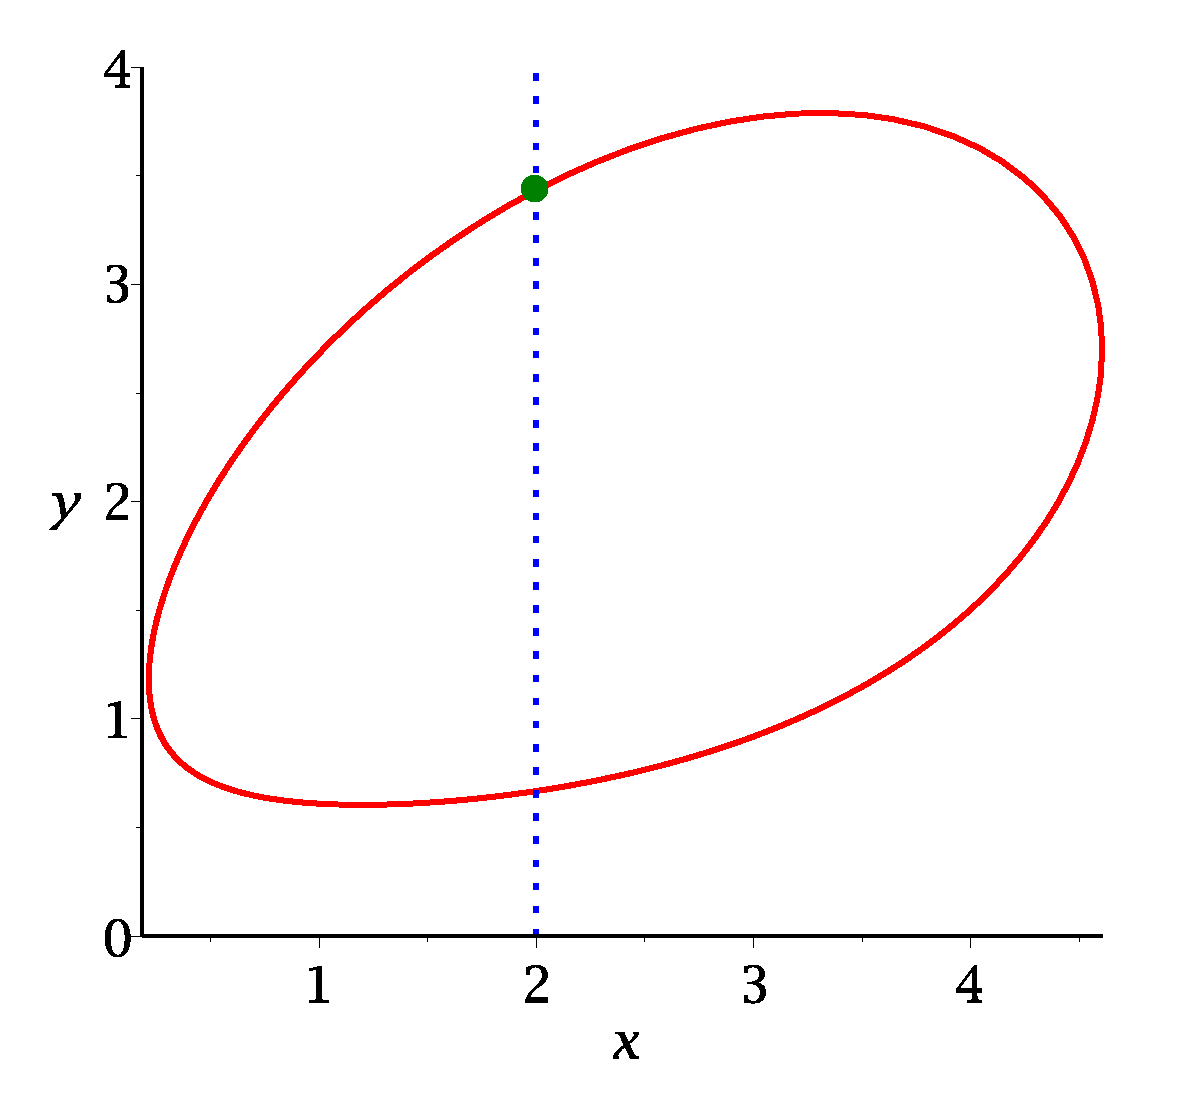
\includegraphics[width=\linewidth]{Images/ex2-op.eps}
    \captionof{figure}{Òrbita periòdica de període $T\simeq 4.1907...$ del sistema \eqref{sist2} (amb $a=1$, $b=-1$ i $c=3/4$) que rodeja l'equilibri $(2,2)$}
    \label{ex2-op}
  \end{minipage}
\end{center}
% \begin{figure}[ht]
%   \centering
%   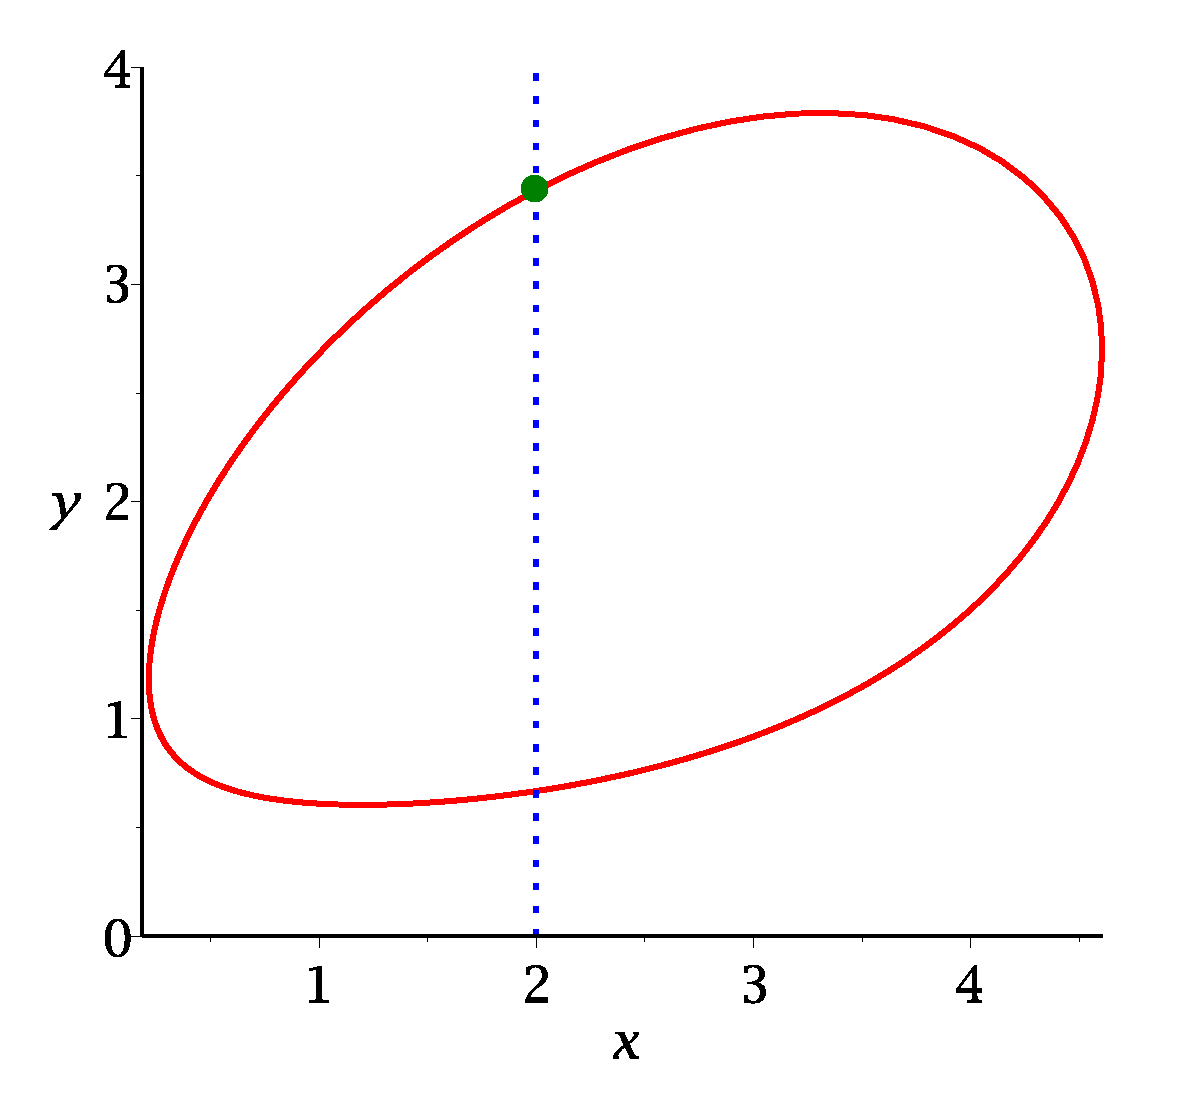
\includegraphics[width=0.4\linewidth]{Images/ex2-op.eps}
%   \caption{Òrbita periòdica del sistema \eqref{sist2} (amb $a=1$, $b=-1$ i $c=3/4$) que rodeja l'equilibri $(2,2)$}
% \end{figure}

L'objectiu ara és fer el mateix fixant dos d'aquests paràmetres i fent variar l'altre en un entorn petit de $(a, b, c) = (1, -1, 3/4)$. És a dir, per a cada valor estudiat dels paràmetres, calcularem la coordenada $y_i$ que és intersecció de l'òrbita periòdica i la recta vertical que passa per l'equilibri al que envolta. A les gràfiques següents s'exposen els resultats obtinguts.

\begin{figure}[ht]
  \centering
  \begin{subfigure}[b]{0.32\linewidth}
    \centering
    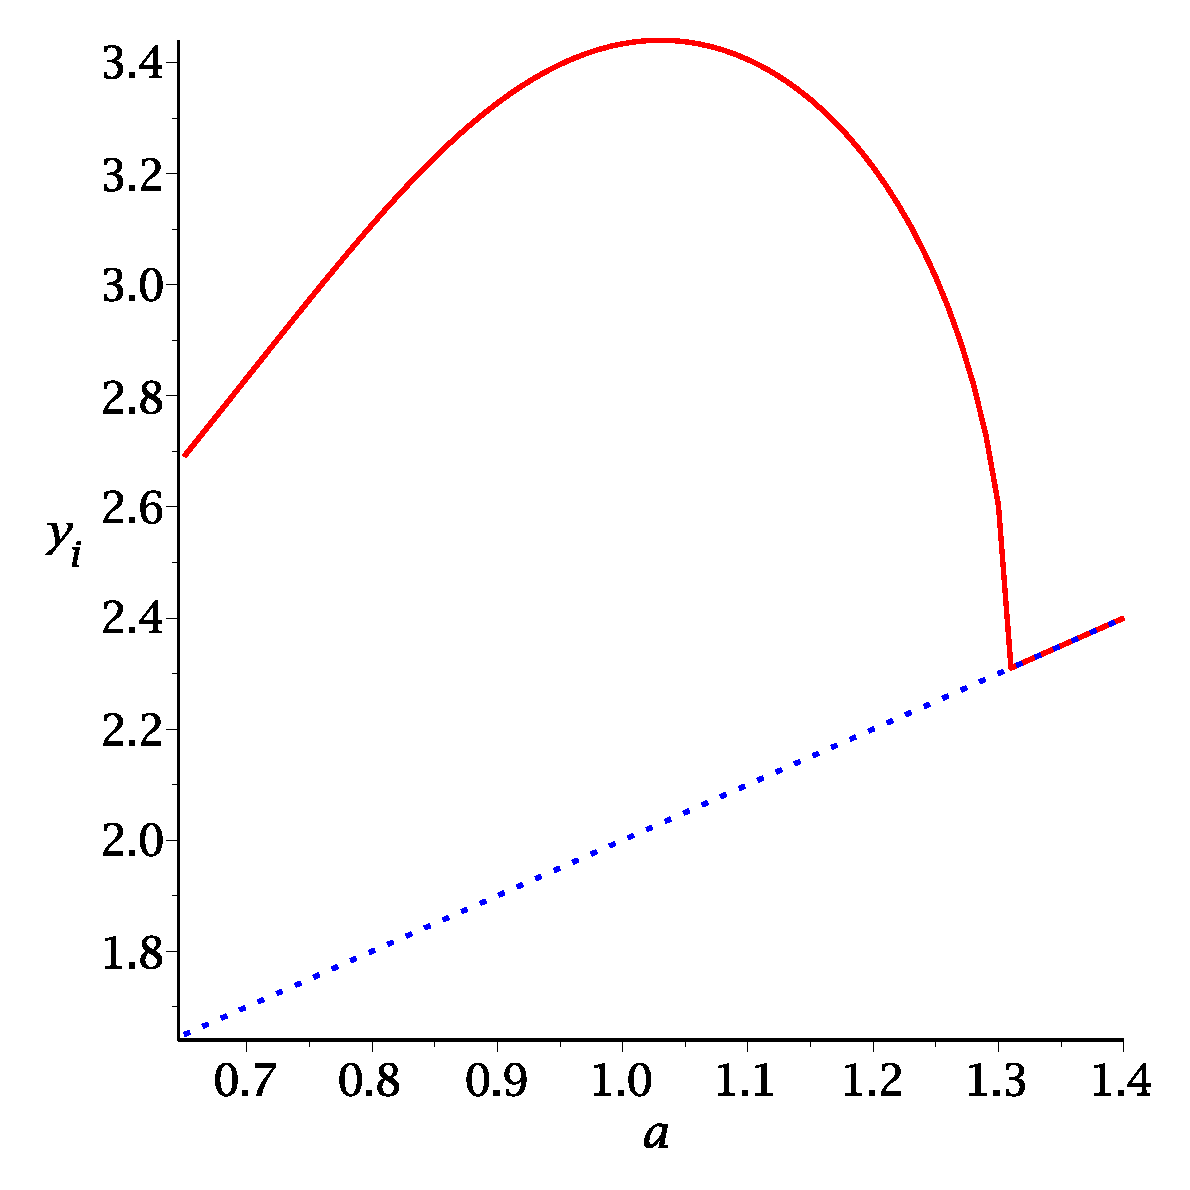
\includegraphics[width=\linewidth]{Images/ex2-a.eps}
    \caption{Gràfic de $y_i$ en funció de $a$}
  \end{subfigure}
  \hfill
  \begin{subfigure}[b]{0.32\linewidth}
    \centering
    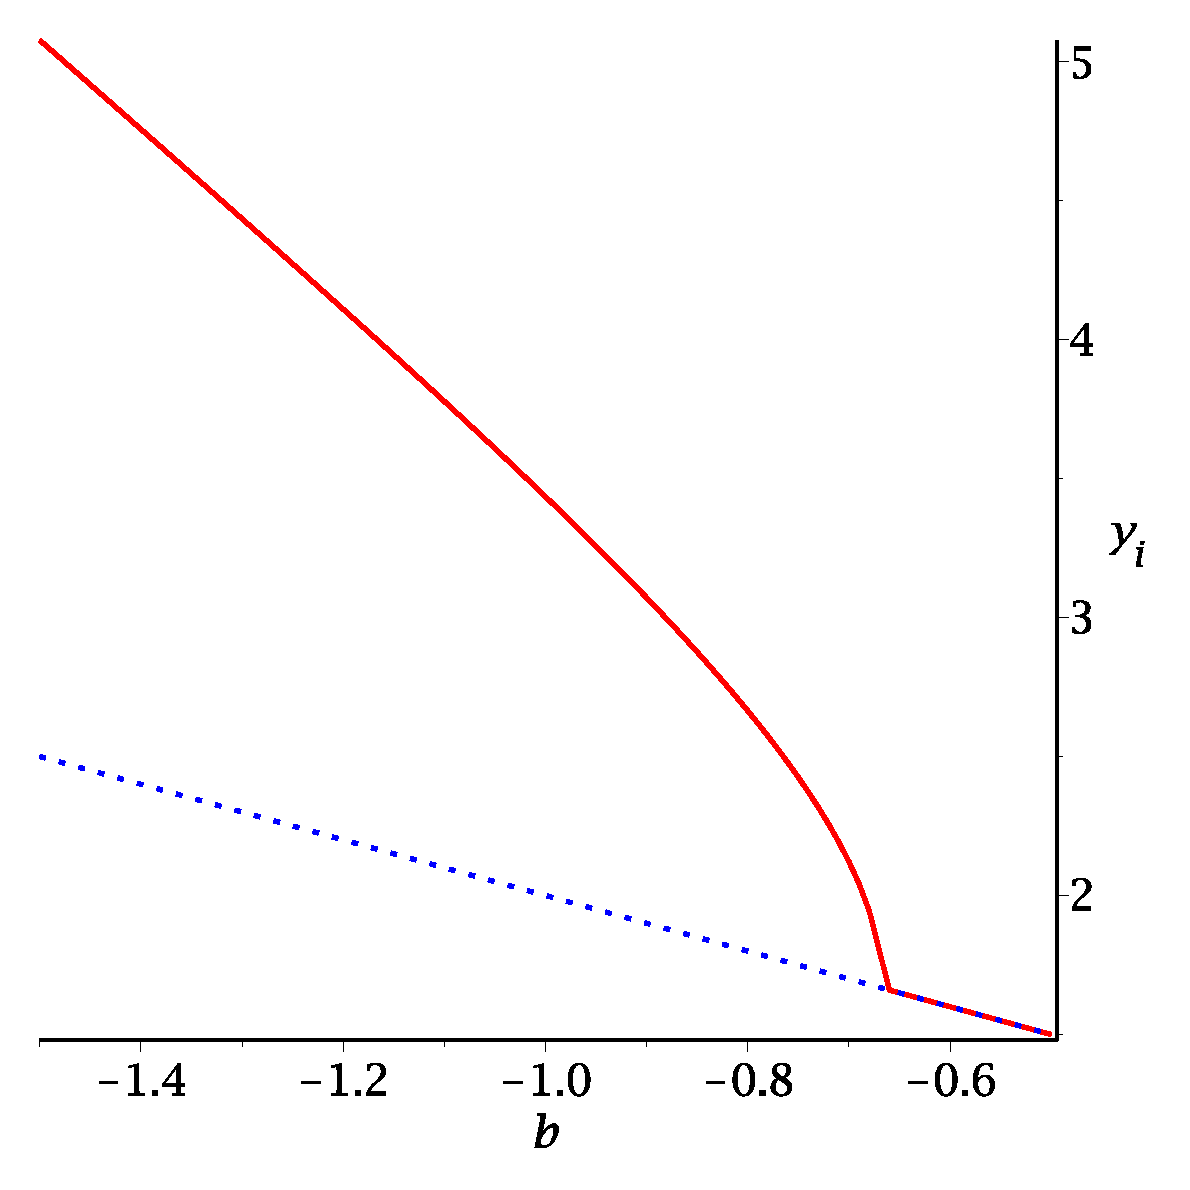
\includegraphics[width=\linewidth]{Images/ex2-b.eps}
    \caption{Gràfic de $y_i$ en funció de $b$}
  \end{subfigure}
  \hfill
  \begin{subfigure}[b]{0.32\linewidth}
    \centering
    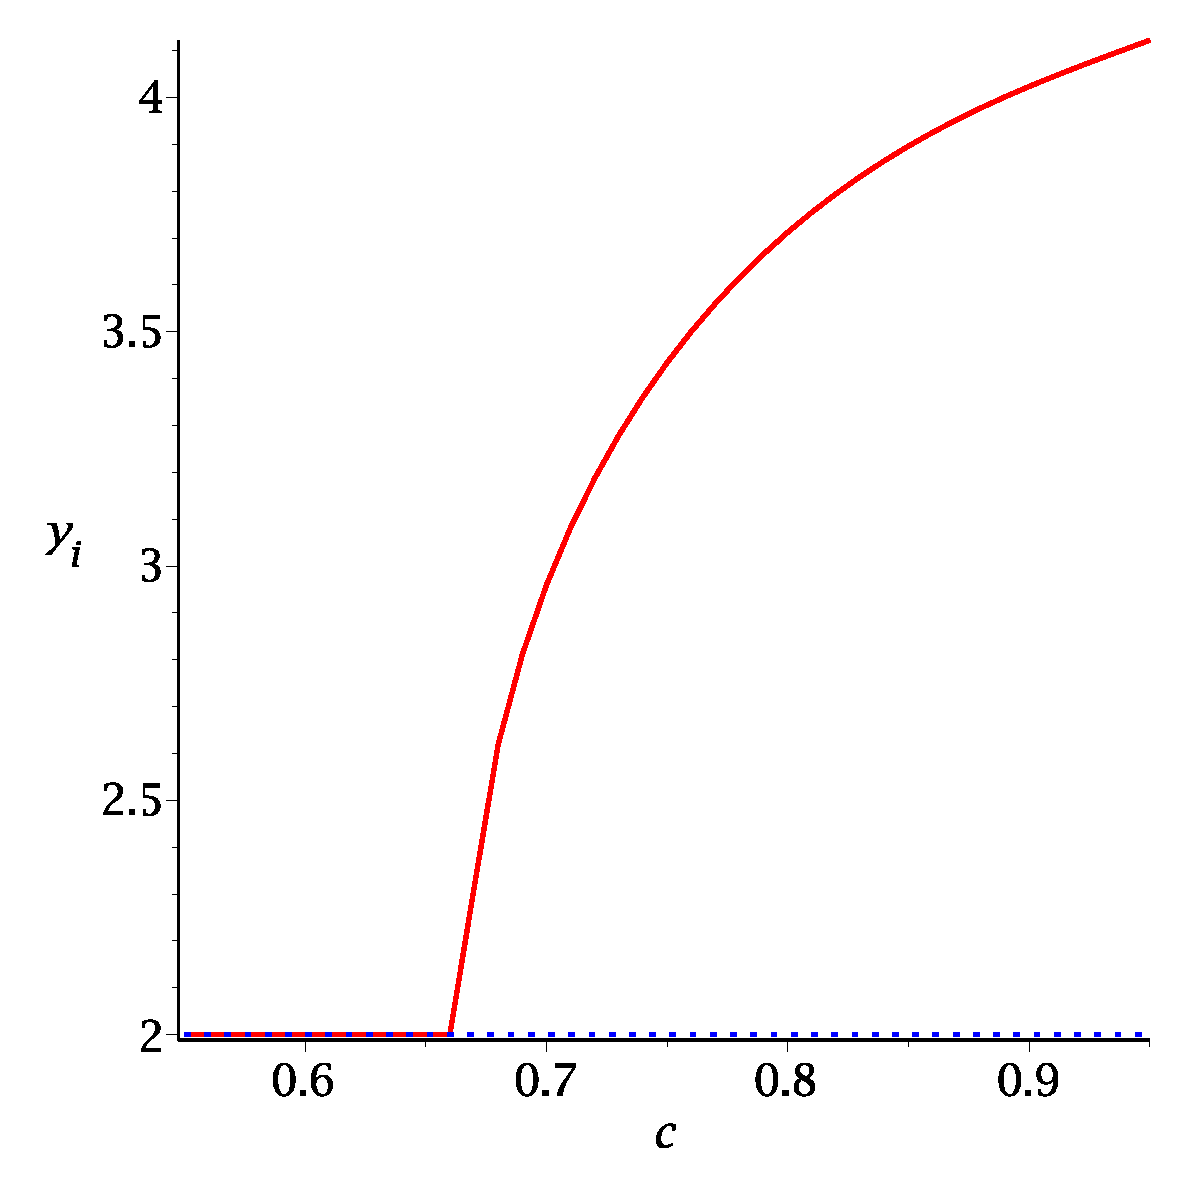
\includegraphics[width=\linewidth]{Images/ex2-c.eps}
    \caption{Gràfic de $y_i$ en funció de $c$}
  \end{subfigure}
  \caption{Gràfics del moviment de la coordenada $y_i$ quan variem cadascun dels paràmetres per separat. La corba vermella indica la coordenada $y_i$ per on passa l'òrbita periòdica mentre que la recta de punts blava indica la coordenada $y$ del punt d'equilibri situat a l'interior d'aquesta.}
\end{figure}

Com bé s'observa en les imatges, l'òrbita periòdica mor en l'equilibri quan variem cadascun dels paràmetres en una certa direcció. Obtenim doncs, bifurcacions de Hopf en cada cas.
\newpage
\section{Òrbites periòdiques a dimensió 3}
Considerem el sistema d'equacions diferencials de Lorenz:
\begin{equation}\label{sist3}
  \left\{
  \begin{aligned}
    x' & = \sigma(-x+y) & =:  g_1(x,y) \\
    y' & = rx-y-xz      & =: g_2(x,y)  \\
    z' & = -bz +xy      & =: g_3(x,y)
  \end{aligned}
  \right.
\end{equation}
Volem estudiar la localització d'òrbites periòdiques. Primer de tot partim del punt $(0, 5, 75)$ amb paràmetres $(b, \sigma, r) = (8/3, 10 , 100.5)$. Com en els casos anteriors, ens caldrà aplicar el mètode de Newton per tal de trobar els zeros de l'aplicació de retorn. Ara, però, la secció transversal que agafem té dimensió 2 i per tant, hem d'utilitzar una versió generalitzada del mètode de Newton, que és la següent. Sigui $\vf{f}:\RR^n\rightarrow\RR^n$ una funció vectorial i $\vf{x}_0\in\RR^n$  una condició inicial. Aleshores els iterats de Newton són:
$$
  \vf{x}_{n+1}=\vf{x}_n - \vf{Df}(x_n)^{-1}\vf{f}(\vf{x}_n)
$$
Així doncs, ens caldrà calcular la diferencial de l'aplicació de Poincaré $\vf{\Pi}$. Si agafem una secció transversal $\{x= s\}$, on $s\in\RR$, aleshores a partir de la equació \eqref{eqPoin} és fàcil adonar-se que:
$$\vf{D\Pi}(y,z)=
  \begin{pmatrix}
    \displaystyle\pdv{\psi_2}{y} - \frac{g_2}{g_1} \pdv{\psi_1}{y} & \displaystyle\pdv{\psi_2}{z} - \frac{g_2}{g_1} \pdv{\psi_1}{z} \\
    \displaystyle\pdv{\psi_3}{y} - \frac{g_3}{g_1} \pdv{\psi_1}{y} & \displaystyle\pdv{\psi_3}{z} - \frac{g_3}{g_1} \pdv{\psi_1}{z}
  \end{pmatrix}
$$
on $\Psi=(\psi_1,\psi_2,\psi_3)$ denota el flux del sistema \eqref{sist3}. Per tant, si anomenem $\vf{d}(y,z)=\vf\Pi(y,z)-(y,z)$ a l'aplicació de retorn, tenim que:
$$\vf{Dd}(y,z)=
  \begin{pmatrix}
    \displaystyle\pdv{\psi_2}{y} - \frac{g_2}{g_1} \pdv{\psi_1}{y} - 1 & \displaystyle\pdv{\psi_2}{z} - \frac{g_2}{g_1} \pdv{\psi_1}{z}    \\
    \displaystyle\pdv{\psi_3}{y} - \frac{g_3}{g_1} \pdv{\psi_1}{y}     & \displaystyle\pdv{\psi_3}{z} - \frac{g_3}{g_1} \pdv{\psi_1}{z} -1
  \end{pmatrix}
$$
Integrant el sistema i iterant amb l'aplicació de Poincaré (fent servir la secció transversal $\{x = 0\}$) trobem finalment una òrbita periòdica que periòdica que passa pel punt $(0,4.2554..., 74.6507...)$ el període de la qual és de $T\simeq 1.0959...$ A la figura \eqref{op3-0} és mostra una representació d'aquesta.

\begin{figure}[ht]
  \centering
  \includegraphics[width=0.4\linewidth]{Images/op3-100.5.pdf}
  \caption{Òrbita periòdica de període $T\simeq 1.0959...$ del sistema de Lorenz amb paràmetres $(b, \sigma, r) = (8/3, 10 , 100.5)$ que passa pel punt  $(x,y,z)=(0,4.2554..., 74.6507...)$}
  \label{op3-0}
\end{figure}

Ara estudiem el cas $r = 25$. Els equilibris en aquest cas són les solucions del sistema d'equacions següent:
\begin{equation*}
  \left\{
  \begin{aligned}
    -x+y              & =  0 \\
    25x-y-xz          & = 0  \\
    -\frac{8}{3}z +xy & =0
  \end{aligned}
  \right.
\end{equation*}
De la primera equació deduïm que $x = y$ i de l'última que $z = \frac{3}{8}x^2$. Substituint això a l'equació restant, tenim que $24x -\frac{3}{8}x^3=0\iff x64(1-x^2)=0$, que té solucions $x=0,\pm 8$. Per tant, els punts d'equilibri són: $(0,0,0)$, $(8,8,24)$ i $(-8,-8,24)$. Ara voldríem estudiar l'existència o no d'òrbites periòdiques en un entorn de cadascun d'aquest equilibris. A continuació mostrem les diferencials del sistema avaluades a cadascun dels punts d'equilibri juntament amb els seus corresponents valors propis:
\begin{align*}
  \vf{Dg}(0,0,0)=\begin{pmatrix}
                   -10 & 10 & 0    \\
                   25  & -1 & 0    \\
                   0   & 0  & -8/3
                 \end{pmatrix}  \qquad\sigma(\vf{Dg}(0,0,0))   & = \begin{bmatrix}
                                                                     10.939... \\ -21.939...\\-2.666...
                                                                   \end{bmatrix}                                 \\
  \vf{Dg}(8,8,24)=\begin{pmatrix}
                    -10 & 10 & 0    \\
                    1   & -1 & -8   \\
                    8   & 8  & -8/3
                  \end{pmatrix} \qquad \sigma(\vf{Dg}(8,8,24))  & = \begin{bmatrix}
                                                                      -13.682... \\ 0.007921...-9.672...\ii\\ 0.007921...+9.672...\ii
                                                                    \end{bmatrix}   \\
  \vf{Dg}(-8,-8,24)=\begin{pmatrix}
                      -10 & 10 & 0    \\
                      1   & -1 & -8   \\
                      8   & 8  & -8/3
                    \end{pmatrix} \qquad\sigma(\vf{Dg}(-8,-8,24)) & = \begin{bmatrix}
                                                                        -13.682... \\ 0.007921...-9.672...\ii\\ 0.007921...+9.672...\ii
                                                                      \end{bmatrix}
\end{align*}
El fet que l'origen tingui direccions propies amb comportament de node ens indica que no hi ha òrbites periòdiques en un entorn petit de l'origen. En canvi, en els altres dos punts crítics tenim valors propis imaginaris, que ens indiquen rotacions del camp. Al haver-n'hi dos tenim dues varietats (dos plans) propies en les quals el camp rota i per tant, on hi pot haver una òrbita periòdica al voltant. Per tant, cal estudiar de forma exhaustiva si aquests equilibris tenen o no òrbites periòdiques al voltant seu. Per això hem partit de la condició inicial $(x_0, y_0, z_0)$ on $x_0=\pm 8$, $y_0\in (\pm 8 - \varepsilon, \pm 8 +\varepsilon)$ i $z_0\in (24 - \varepsilon, 24 +\varepsilon)$ i $\varepsilon\in[0,16]$. Així doncs, partint de la secció transversal $\{x=\pm 8\}$ hem calculat el valor de l'aplicació de retorn en cadascun dels punts en l'entorn mencionat. A les següents gràfiques es mostren els resultats obtinguts:

\begin{figure}[ht]
  \centering
  \begin{subfigure}[b]{0.45\linewidth}
    \centering
    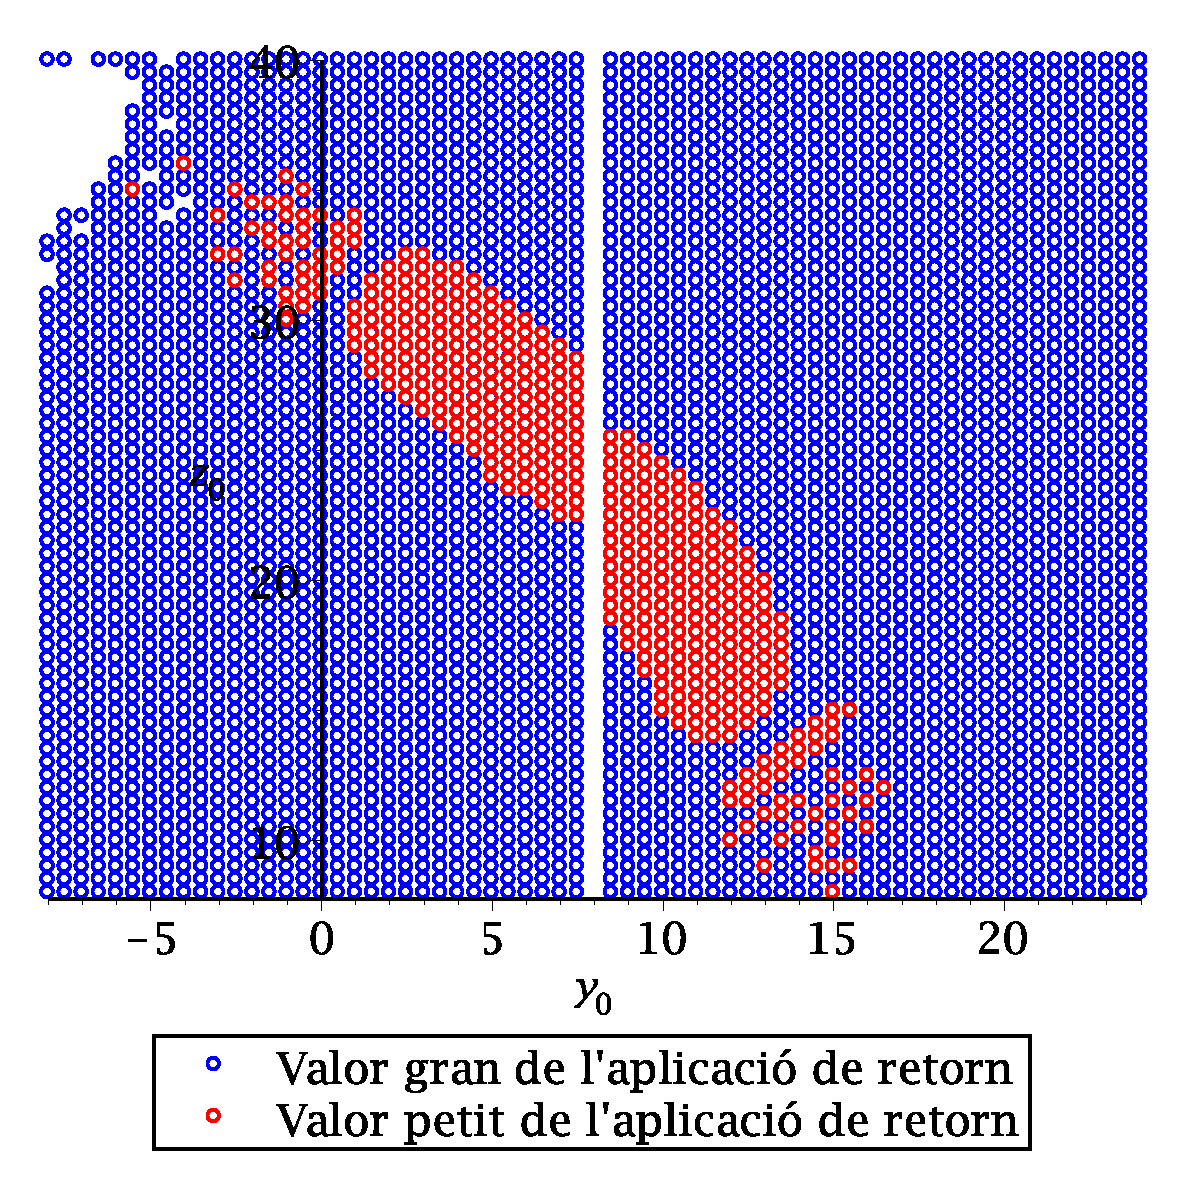
\includegraphics[width=\linewidth]{Images/ex3-8vb.eps}
    \caption{Anàlisi per $x_0 = 8$}
  \end{subfigure}
  \hfill
  \begin{subfigure}[b]{0.45\linewidth}
    \centering
    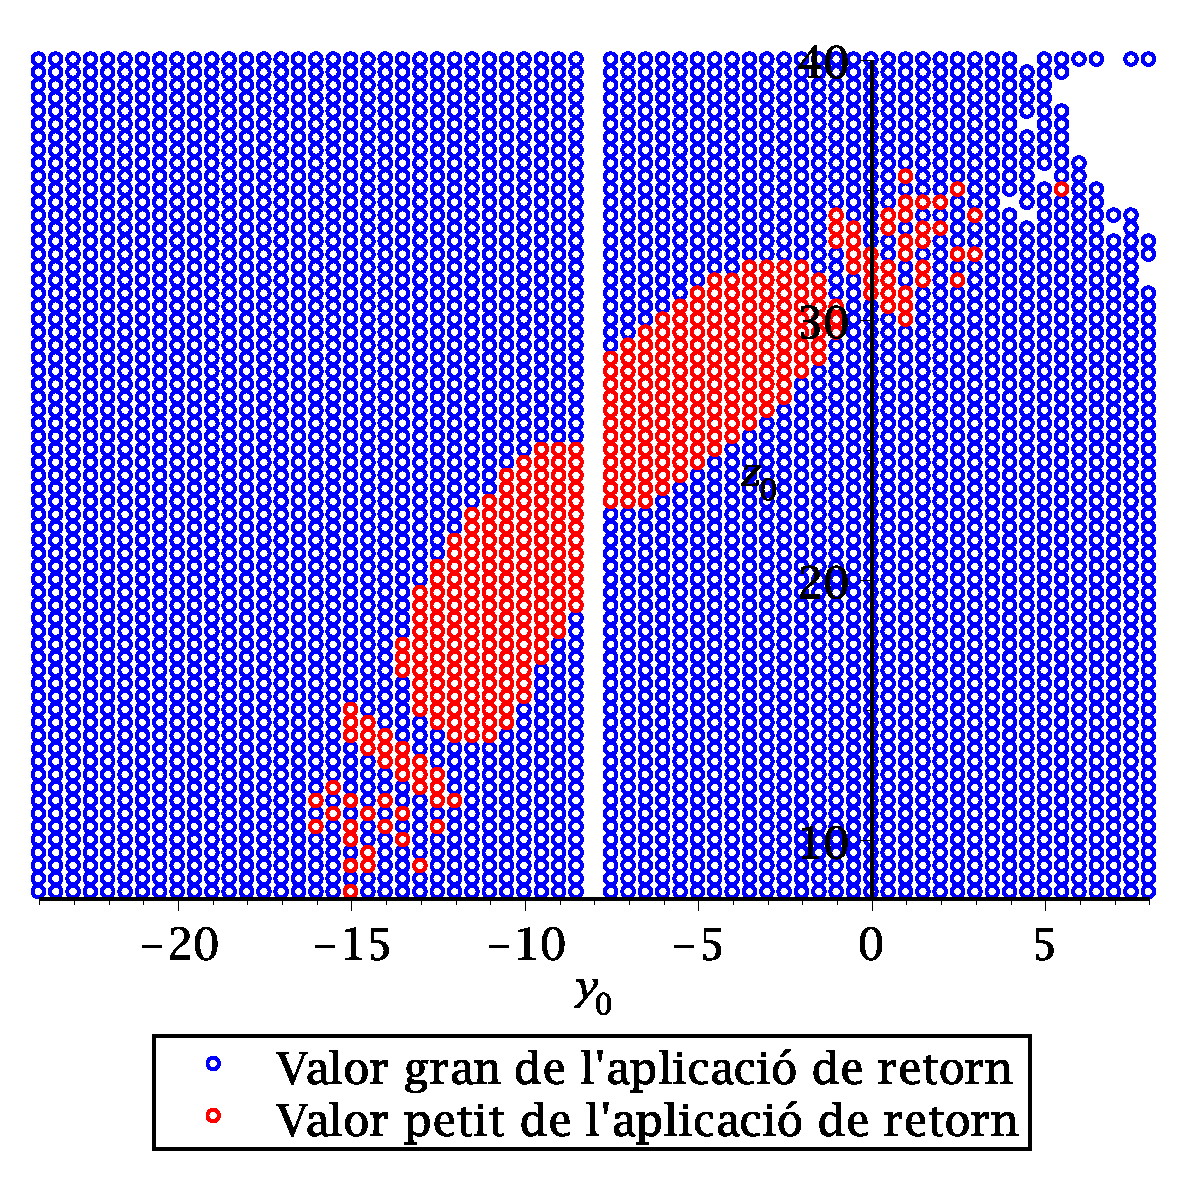
\includegraphics[width=\linewidth]{Images/ex3--8vb.eps}
    \caption{Anàlisi per $x_0 = - 8$}
  \end{subfigure}
  \caption{Gràfic que ens mostra la distància de l'aplicació de retorn conforme integrem el sistema de Lorenz partint de diverses condicions inicial. Els punts vermells indiquen un valor de $\vf{d}$ ``petit'' mentre que els punts blaus indiquen un valor de $\vf{d}$ ``gran''. }
\end{figure}

Notem que els punts no graficats han estat e\lgem iminats per problemes computacionals. A més les dues bandes vermelles que s'observen al mig de les imatges no són significatives, en el sentit de ser possibles candidats a ser condicions inicials d'òrbites periòdiques, ja que es deu a la forta rotació del camp al voltant dels dos equilibris. El naixement de les òrbites periòdiques el trobem als punts discrets que ``estenen'' aquesta banda central. És interessant observar també la simetria dels gràfics. A més en cada gràfic els punts discrets de dalt i els punts discrets de baix corresponen, cadascun amb el seu simètric, a la mateixa òrbita periòdica.

Si partim de cadascuna d'aquestes condicions inicials especials de color vermell, obtenim algunes de les òrbites periòdiques que s'exposen a la figura \ref{op3-25}. Observant les figures podem contrastar la simetria que ens referíem anteriorment. Quan partim de $x_0=8$ les òrbites periòdiques fan més voltes al voltant de l'altre punt d'equilibri situat a $x=-8$ i viceversa. Únicament coincideixen quan aquestes només fan una volta al voltant de l'altre equilibri (gràfics \ref{fig2} i \ref{fig5}).

% \vspace{5cm}

\begin{figure}[ht]
  \captionsetup[subfigure]{justification=centering}
  \centering
  \begin{subfigure}[b]{0.45\linewidth}
    \centering
    \includegraphics[width=0.95\linewidth]{Images/op3-25-1.pdf}
    \caption{Condició inicial: $(8, 14.356..., 10.737...)$\\ Període: $3.277...$}
  \end{subfigure}
  \hfill
  \begin{subfigure}[b]{0.45\linewidth}
    \centering
    \includegraphics[width=0.95\linewidth]{Images/op3-25-2.pdf}
    \caption{Condició inicial: $(8, 0.002224..., 32.173...)$\\ Període: $1.693...$}
    \label{fig2}
  \end{subfigure}
  \\
  \centering
  \begin{subfigure}[b]{0.45\linewidth}
    \centering
    \includegraphics[width=0.95\linewidth]{Images/op3-25-3.pdf}
    \caption{Condició inicial: $(8, -2.365..., 33.915...)$\\ Període: $4.778...$}
  \end{subfigure}
  \hfill
  \begin{subfigure}[b]{0.45\linewidth}
    \centering
    \includegraphics[width=0.95\linewidth]{Images/op3-25-4.pdf}
    \caption{Condició inicial: $(-8, -14.356..., 10.737...)$\\ Període: $3.277...$}
  \end{subfigure}\\
  \begin{subfigure}[b]{0.45\linewidth}
    \centering
    \includegraphics[width=0.95\linewidth]{Images/op3-25-5.pdf}
    \caption{Condició inicial: $(-8, -0.002224..., 32.173...)$\\ Període: $1.693...$}
    \label{fig5}
  \end{subfigure}
  \hfill
  \begin{subfigure}[b]{0.45\linewidth}
    \centering
    \includegraphics[width=0.95\linewidth]{Images/op3-25-6.pdf}
    \caption{Condició inicial: $(-8, 2.365..., 33.915...)$\\ Període: $4.778...$}
  \end{subfigure}
  \caption{Algunes de les òrbites periòdiques del sistema de Lorenz amb coeficients $(b,\sigma, r)=(8/3, 10 , 25)$}
  \label{op3-25}
\end{figure}
\end{document}

